\subsection{ソフトウェアエンジニアリング運用制御}

運用制御は、運用中のサービスを観察し、制御し、問題に対応し、変更を管理し、結果を報告する活動である。運用は一度設定すれば終わりではない。利用者、負荷、脅威、法規制、事業要求、技術基盤は変化する。その変化を制御しなければ、サービス品質は低下する。

\subsubsection{インシデント管理}

インシデント管理とは、ソフトウェアインシデントを記録し、優先順位を付け、事業影響を評価し、解決、エスカレーション、終了まで管理するプロセスである。

現代のDevOpsでは、アラートとログを用いた監視を自動化し、小さなインシデントが大きな障害になる前に検出する。インシデントが発生したら、原因を分析し、事後検討を行い、同じインシデントを繰り返さないための対策を実施する。

\subsubsection{変更管理}

変更管理とは、すべての変更を評価、承認、実装、レビューされた状態で行うためのプロセスである。変更要求は記録され、緊急、至急、重大、軽微などに分類される。変更管理では、変更のリスク、ロールバック戦略の必要性、関係者への通知、変更スケジュールを扱う。

従来型の開発では、多くの変更をまとめて定期リリースとして提供することが多かった。DevOpsでは、小さな変更単位を独立に、必要に応じて届けることを目指す。そのためには、ソフトウェアが小さく独立した配備に向くように設計されている必要がある。

\subsubsection{監視、測定、追跡、レビュー}

運用では、容量、継続性、可用性を監視する。DevOpsの考え方では、希望的観測に頼ってはならない。システム品質と運用状態を、証拠に基づいて判断する必要がある。

\par\smallskip\noindent\refstepcounter{table}\label{tab:ch06-07}\textbf{表 \thetable: 第06章 ソフトウェアエンジニアリング運用 表07}\par\smallskip
\begin{longtable}{L{55mm}L{95mm}}
\toprule
測定対象 & 意味 \\
\midrule
本番システム監視と製品テレメトリ & 本番で何が起きているかを示す。ログ、トレース、利用者行動、資源使用量などを含む。 \\
リリース前後の検証結果 & リリースが期待どおりに動くか、リリース後に品質が悪化していないかを示す。 \\
利用者活動と資源使用 & どの機能が使われ、どの資源が消費されているかを示す。 \\
影響分析結果 & ある変更がどの機能、構成、利用者に影響するかを示す。 \\
依存関係 & サービス運用に必要な内部依存と外部依存を示す。 \\
構成変更 & 承認済み配備以外の設定変更や環境差分を検出する。 \\
セキュリティと耐障害性 & 攻撃、障害、復旧に対する能力を示す。 \\
\bottomrule
\end{longtable}

\begin{figure}[htbp]
\centering
\IfFileExists{assets/generated_figures/ch06/fig-ch06-09.png}{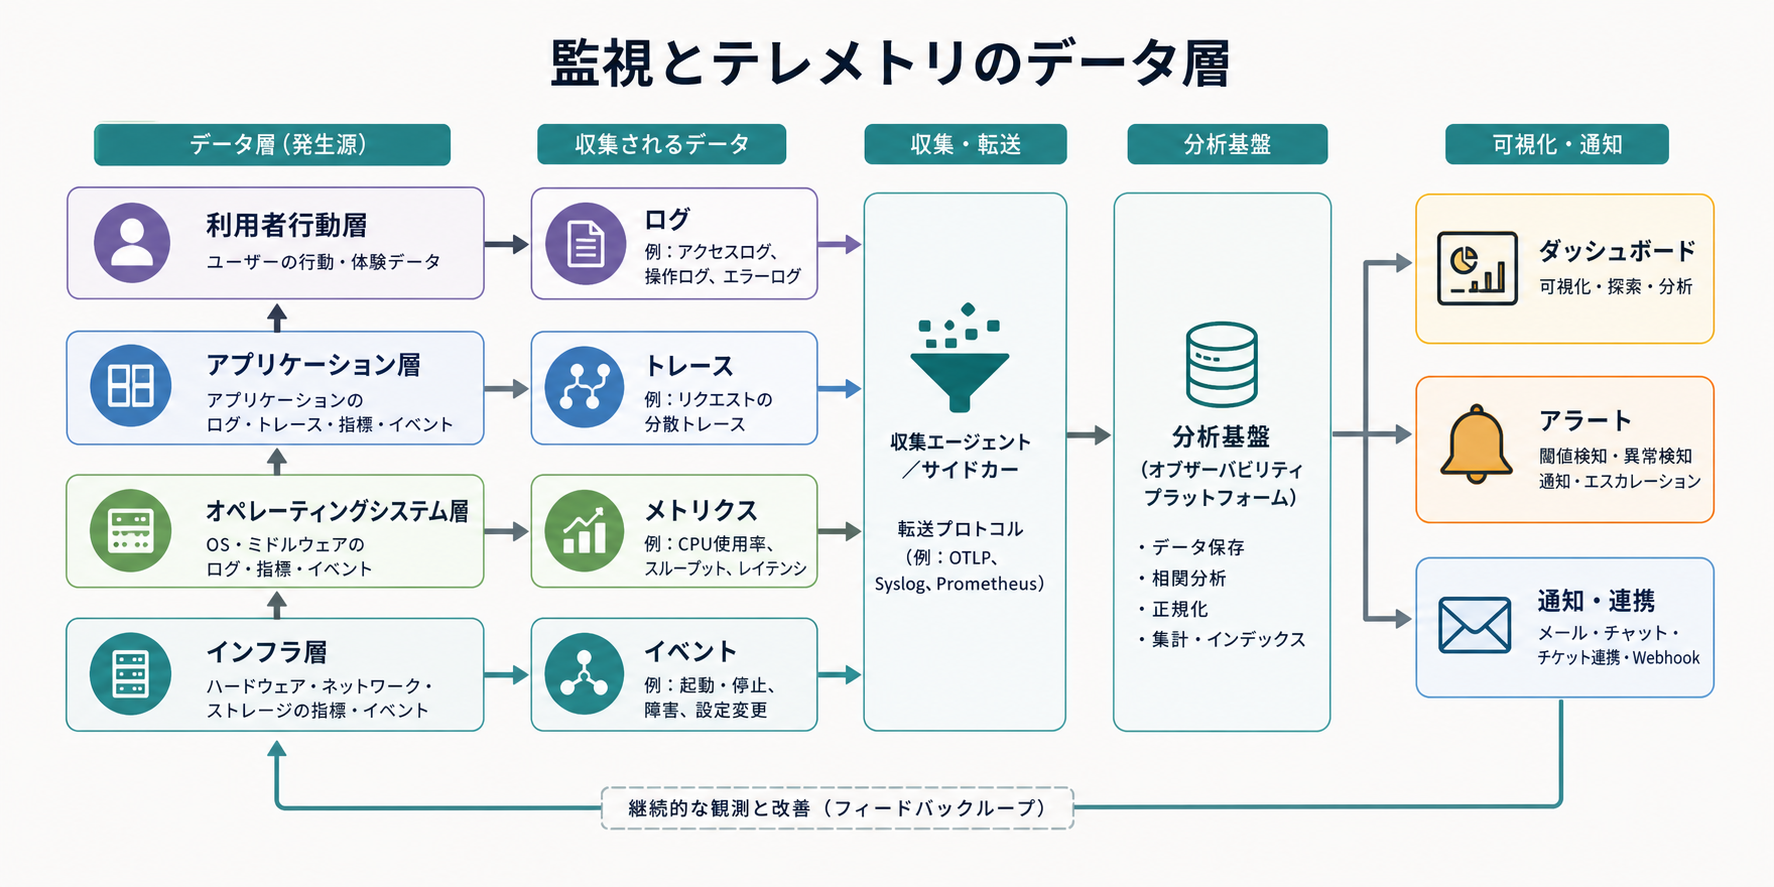
\includegraphics[width=0.96\linewidth]{assets/generated_figures/ch06/fig-ch06-09.png}}{\fbox{\parbox[c][48mm][c]{0.9\linewidth}{\centering 画像生成待ち\\監視とテレメトリのデータ層}}}
\caption{監視とテレメトリのデータ層}
\label{fig:ch06-09}
\end{figure}

\subsubsection{運用支援}

運用支援は、ソフトウェア製品を意図された環境で動かし、顧客や利用者を支援する活動である。運用支援はプロジェクトの計画段階から始まり、実行段階では監視、イベント対応、インシデント対応、問い合わせ対応、手順実行、運用文書更新を行う。

運用支援活動はSLAに記述されることが多い。たとえば、サポート時間、初動応答時間、障害の重大度分類、復旧目標、報告形式、エスカレーション経路などである。

\subsubsection{サービス報告}

サービス報告は、意思決定に必要な、合意済みで、適時で、信頼でき、正確な情報を作る活動である。報告は、運用サービスがどのように機能したか、サービス水準を満たしたか、どの問題が発生したか、今後の傾向がどうかを示す。

典型的な報告項目には、サービス水準目標に対する性能、セキュリティ侵害、トランザクション量、資源使用量、インシデントと失敗、傾向情報、満足度分析がある。測定を自動化し、収集、分析、報告、制御を調整できる枠組みとツールを選定することが重要である。

\begin{figure}[htbp]
\centering
\IfFileExists{assets/generated_figures/ch06/fig-ch06-10.png}{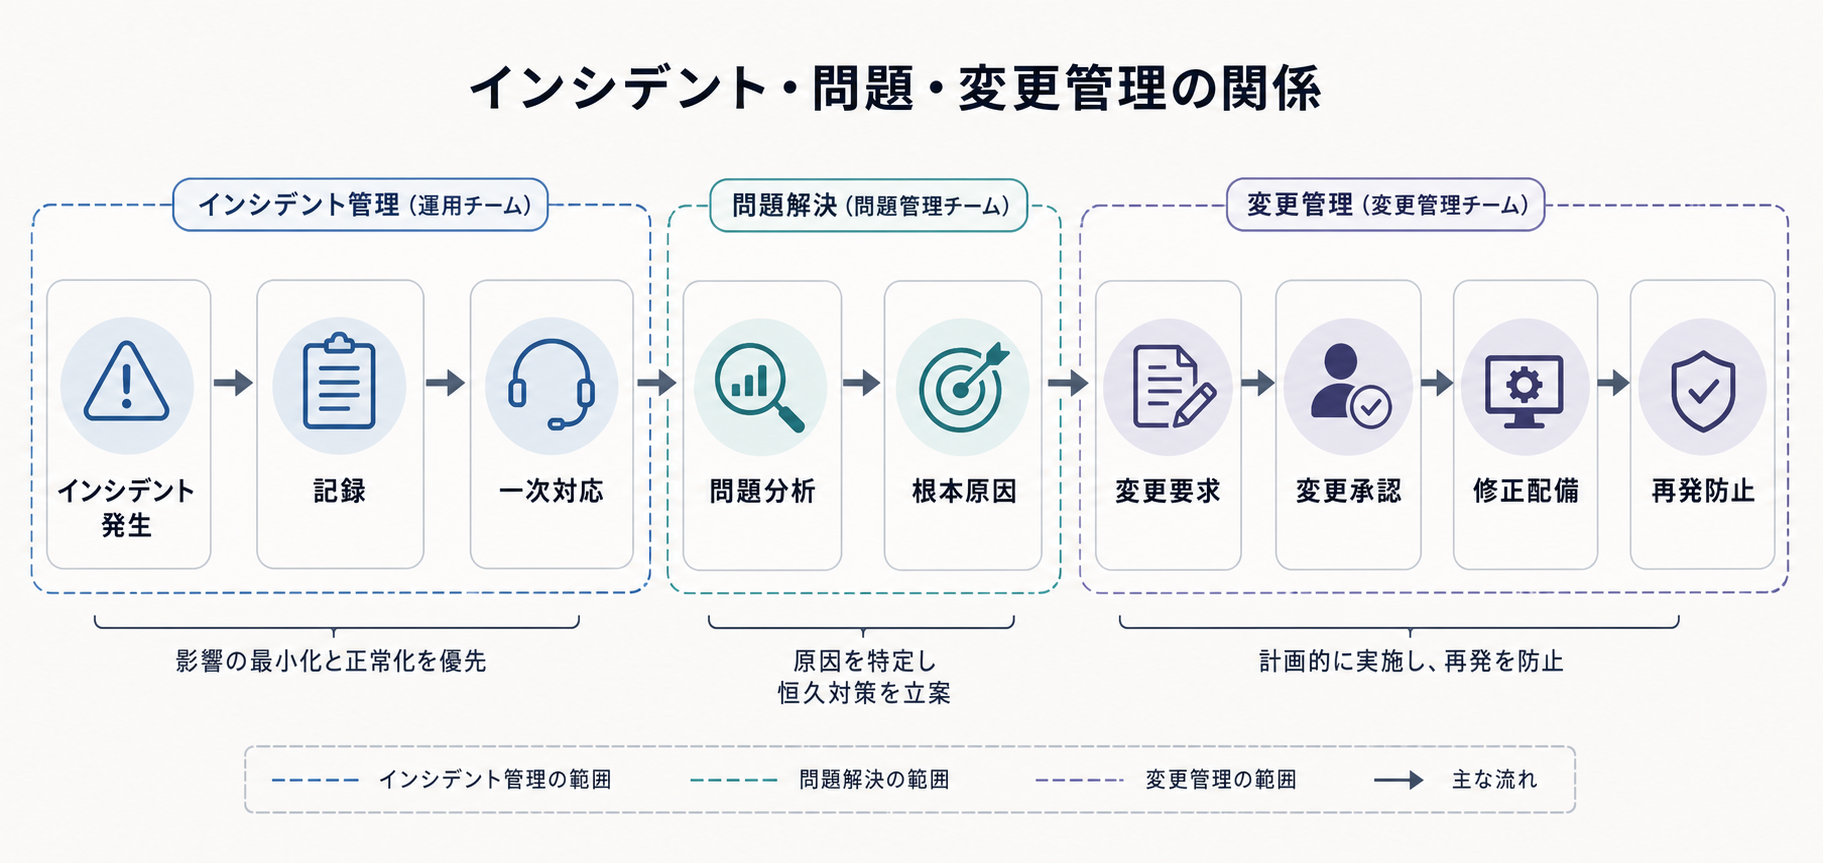
\includegraphics[width=0.96\linewidth]{assets/generated_figures/ch06/fig-ch06-10.png}}{\fbox{\parbox[c][48mm][c]{0.9\linewidth}{\centering 画像生成待ち\\インシデント・問題・変更管理の関係}}}
\caption{インシデント・問題・変更管理の関係}
\label{fig:ch06-10}
\end{figure}
